% !TEX ../report.tex

fonctionnalités et captures aussi sur tablette !

Lors de la première utilisation d'application, l'utilisateur doit choisir son master password. Ce mot de passe servira à chiffrer le fichier de sauvegarde qui contiendra tous les mots de passe l'utilisateur.

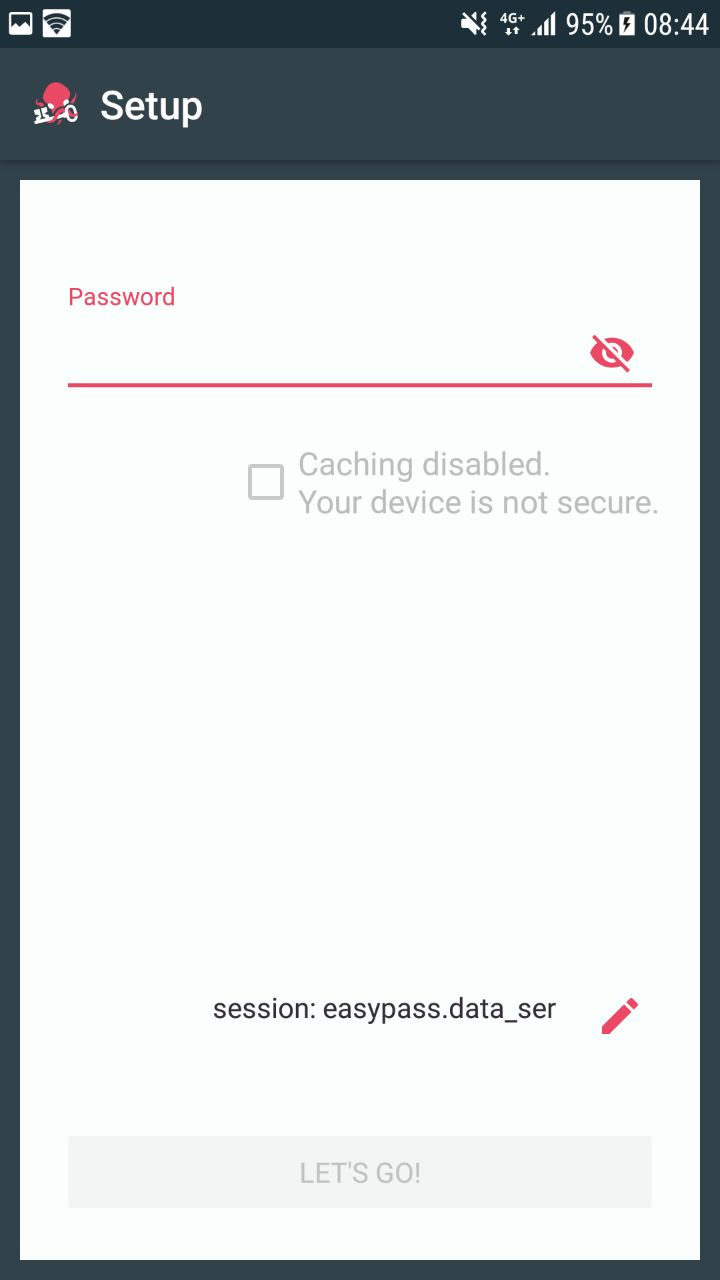
\includegraphics[height=10cm]{login.jpg}

L'utilisateur doit également autoriser l'accès de l'application à Dropbox.
L'application débute avec la vue login. Le master password est demandé afin de déchiffrer le fichier de sauvegarde des mots de passe. Ce mot de passe doit être compliqué afin de garantir la sécurité de l'application. Afin d'améliorer l'expérience utilisateur, l'application \easypass{} lui propose de le mettre en cache et d'utiliser les méthodes d'authifications fournies par Android.

L'application affiche le fichier utilisé pour sauvegarder les mots de passe. Il est possible de modifier le fichier selectionné.

La vue principale ou l'activité principale affiche la liste de tous les comptes de l'utilisateur. L'utilisateur peut ajouter un nouveau compte grâce au bouton flottant.

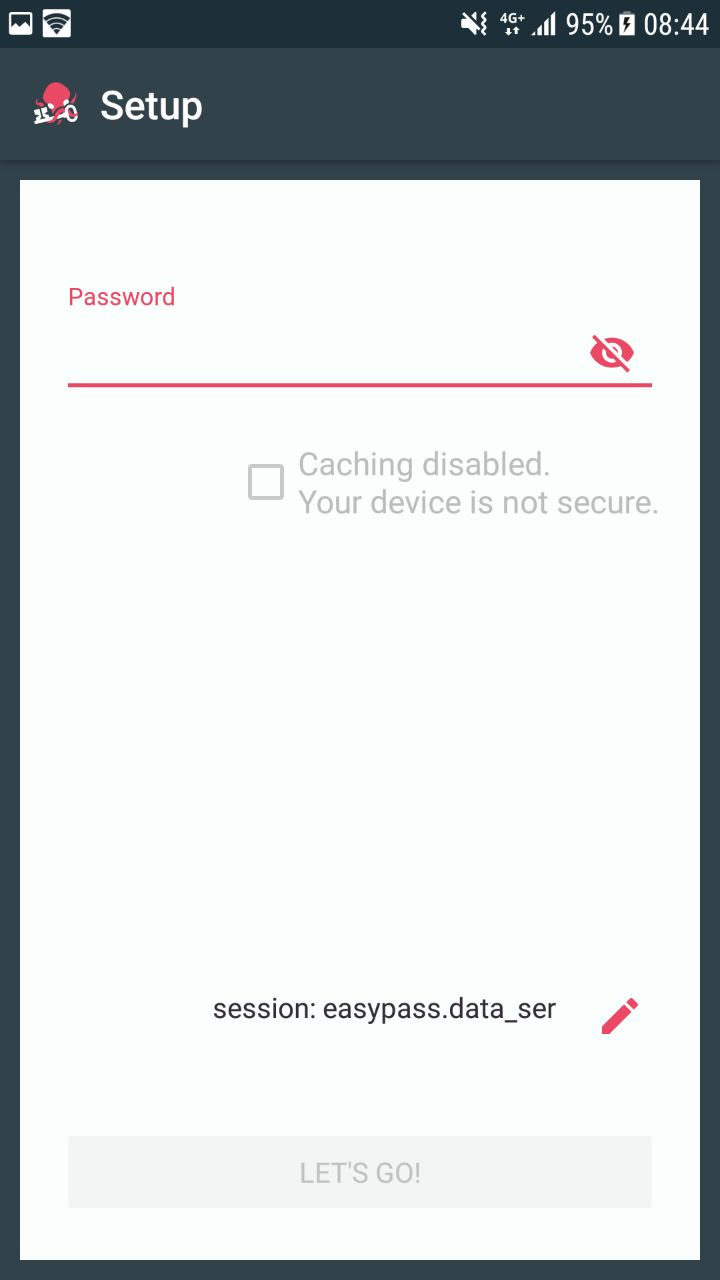
\includegraphics[height=10cm]{login.jpg}

Différentes informations peuvent être spécifiées pour le compte ainsi que le mot de passe. L'application \easypass{} propose également de générer un password aléatoire.

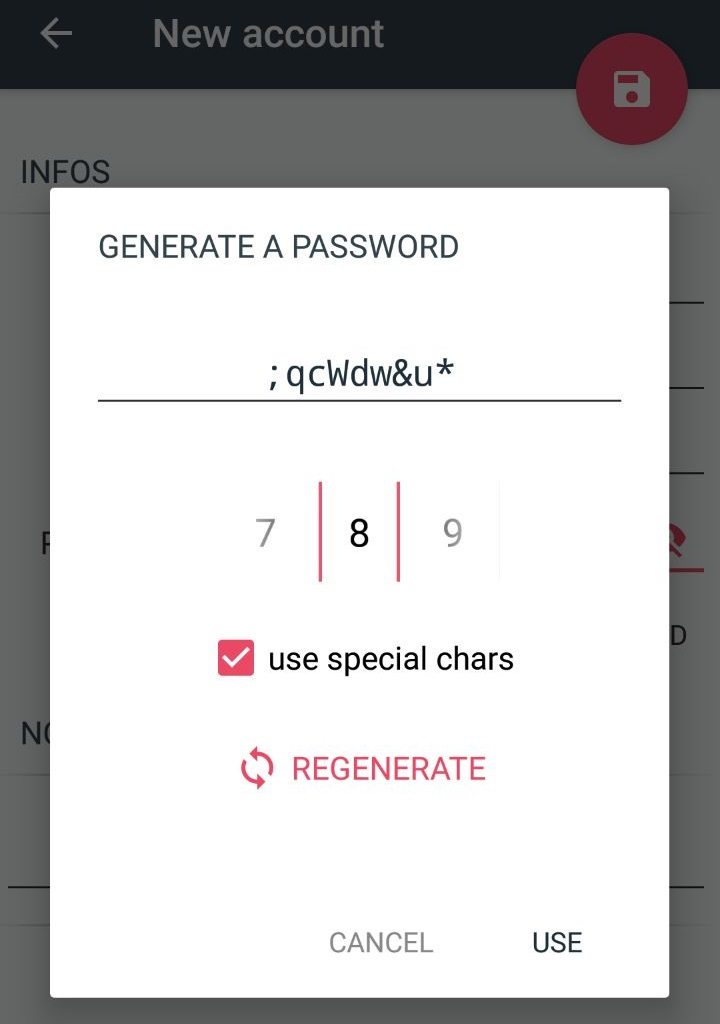
\includegraphics[height=7cm]{generate_password.jpg}

L'utilisateur peut générer un password aléatoire selon différents critères. La liste des caractères spéciaux utilisés peut être configurée dans les settings de l'application.

 L'objectif dans de l'application \easypass{} est de permettre à l'utilisateur de trouver le plus rapidement possible les informations du compte qu'il recherche. La liste affichée peut être triée par ordre et ordre inverse alphabetanumerique ou par date de création. Une fonction recherche est également proposé pour retrouver le nom du compte. Les comptes les plus utilisés peutvent être selectionnés par l'utilisateurs. Ils apparaitront en haut de la liste. 

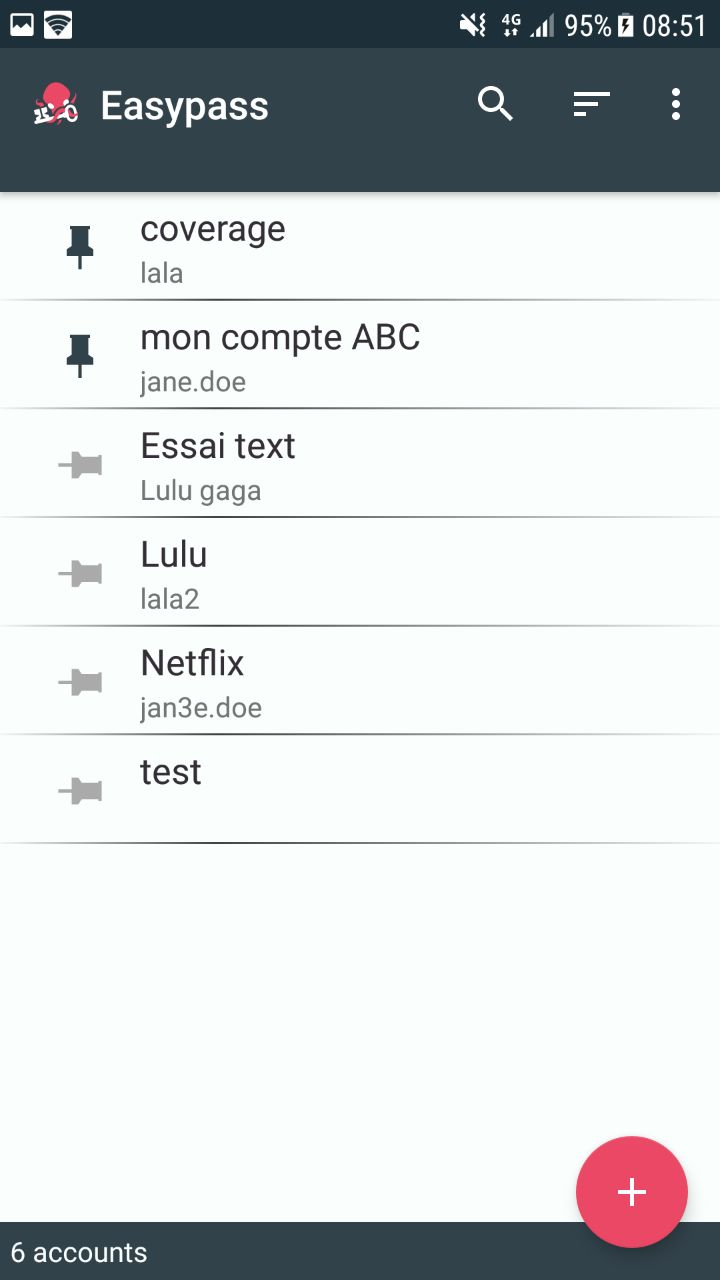
\includegraphics[height=10cm]{liste.jpg}

Lorsque l'utilisateur selectionne un compte, il peut voir dans le pannel toutes les opérations possible : 
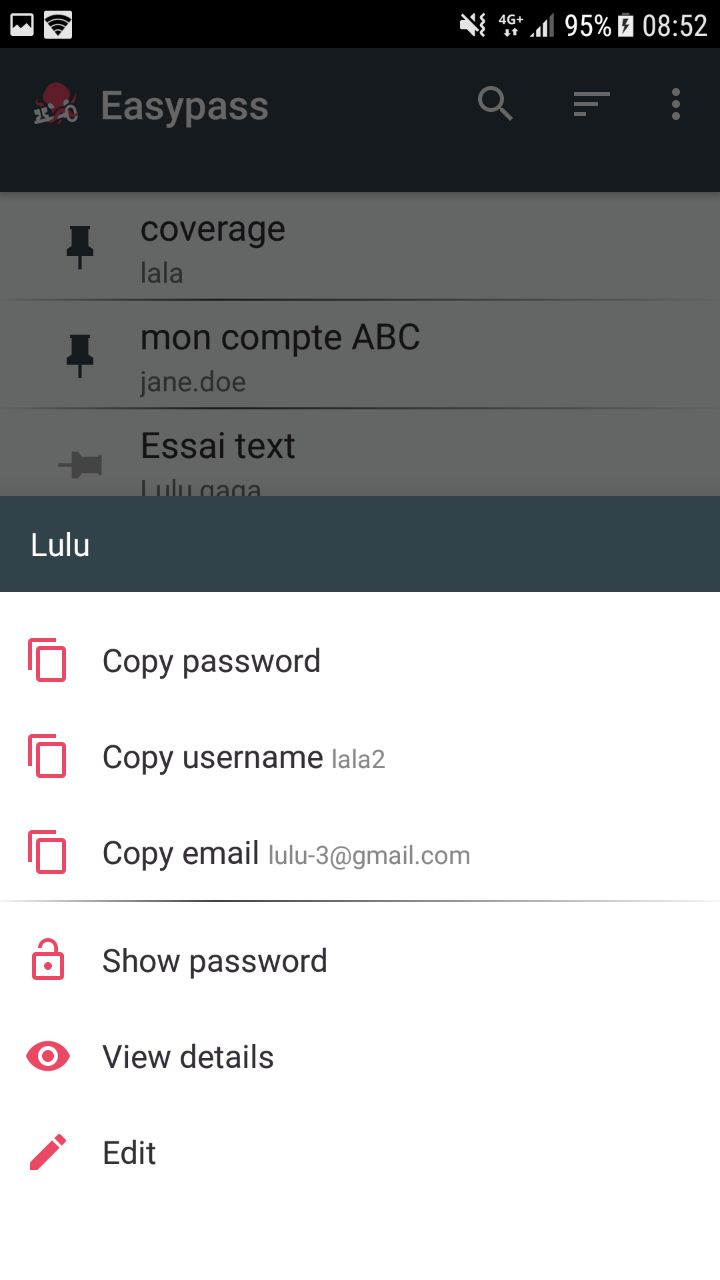
\includegraphics[height=10cm]{liste-edition.jpg}

Toujours dans un soucis d'améliorer l'expérieuce utilisateur, le pannel offre des raccourcis tel que copy email ou view password. Toutes les informations du compte sont disponibles dans la vue détail.

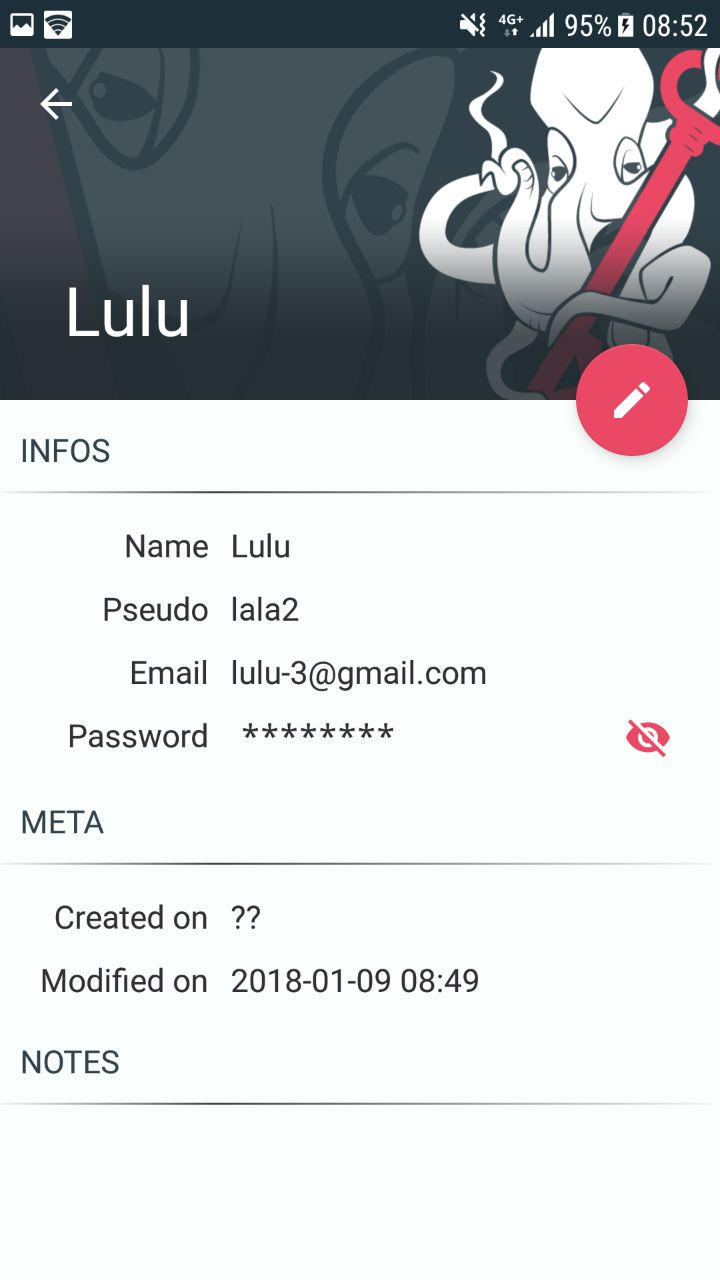
\includegraphics[height=10cm]{details.jpg}

Les options de configuration et personalisation sont disponible dans la vue settings atteignable depuis la vue principale. L'utilisateur peut ici configurer le master password et gérer le fichier synchroniser dans Dropbox.

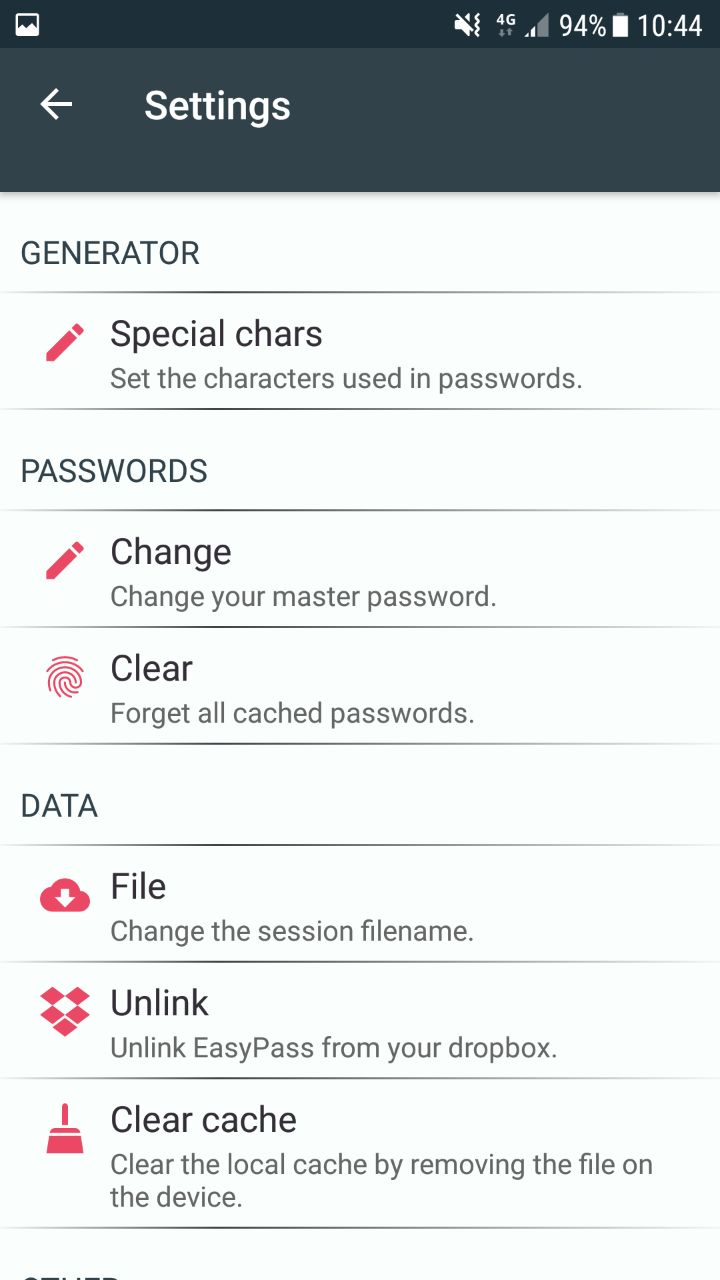
\includegraphics[height=10cm]{settings.jpg}

% exemple multiple images horizontal
\begin{center}
    \begin{minipage}{.3\textwidth}
        \includeFigure{1}{login}{Login 1}
    \end{minipage}
    \begin{minipage}{.3\textwidth}
        \includeFigure{1}{login}{Login 2}
    \end{minipage}
    \begin{minipage}{.3\textwidth}
        \includeFigure{1}{login}{Login 3}
    \end{minipage}        
\end{center}

% exemple de référence
blabla (see Figure \ref{fig:login}) blabla.

% exemple 1 figure
\includeFigure{.5}{generate_password}{caption text}